\documentclass[a4paper,11pt]{article}

\usepackage[margin=22mm]{geometry}
\usepackage{graphicx}
\graphicspath{{../../}{../}{./}}
\usepackage{booktabs}
\usepackage{array}
\usepackage{tabularx}
\usepackage{float}
\usepackage{caption}
\usepackage{hyperref}
\usepackage{zxjatype}
\usepackage[haranoaji]{zxjafont}

\setlength{\parindent}{0pt}
\setlength{\parskip}{0.45em}
\renewcommand{\arraystretch}{1.15}
\newcolumntype{L}[1]{>{\raggedright\arraybackslash}p{#1}}
\newcommand{\reraptor}{ReRAPTOR}

\begin{document}

\sloppy

\title{ReRAPTOR の実験結果整理（更新版）}
\author{Bin Zhou}
\date{2026年4月14日}
\maketitle

\tableofcontents

\section{更新版について}
この文書は，先生に先に見ていただくための実験整理メモの更新版です．
この文書では現在の実験体系だけを扱う形に整理しました．

現時点で main tree に残している実験は，次の 4 本です．

\begin{table}[H]
    \centering
    \small
    \caption{今回の文書で扱う現在の実験体系}
    \begin{tabularx}{\linewidth}{L{1.4cm}L{4.0cm}X}
        \toprule
        実験 & 役割 & 今回の主な読み方 \\
        \midrule
        実験1 & score-guided benchmark & 主タスクで本手法が baseline より高い stop score を出せるか，かつ runtime が現実的かを確認する \\
        実験2 & pruning ablation & Beam / Dominance / Negative の 3 層が，それぞれ何に効いているかを分解して確認する \\
        実験3 & quality-speed balance & 「平均 score が高い」だけでなく，quality と runtime のバランスでも説明できるかを確認する \\
        実験4 & route case study & 実験1・3で得た定量差を，具体的な route の形として視覚的に読めるようにする \\
        \bottomrule
    \end{tabularx}
\end{table}

今回の更新版で私が一番強く言えそうだと思っているポイントは，次の 3 点です．
\begin{itemize}
    \item score-guided 主タスクでは，\reraptor{} が平均 stop score でも quality-speed balance でも最も説明しやすい位置にある．
    \item pruning の中では Dominance が最も本質的であり，Beam は高 budget 条件での安定化，Negative は theme-oriented task における route 整合性の維持として読むのが自然である．
    \item 現在の Experiment 4 は，旧版のような追加 benchmark ではなく，主張を具体例で補強する qualitative case study として置く方が論文全体の流れに合う．
\end{itemize}

\section{実験1：score-guided benchmark}
\subsection*{目的}
実験1の目的は，現在の主タスク
「固定 budget 内で，訪れた stop に割り当てられた score の総和を最大化する」
という setting において，
\reraptor{} が代表的 baseline より高い価値の route を返せるかを確認することです．
ここでは特に，
\textbf{(1) 平均 stop score が高いか}，
\textbf{(2) その改善が極端に遅い探索の上に成り立っていないか}，
\textbf{(3) 4h / 8h や score seed を変えても傾向が保たれるか}
を見ています．

\subsection*{実験設定}
データは福岡市 GTFS をベースにした同一ネットワークを用いています．
探索条件は，
10 origins，
3 departure times（07:00 / 10:00 / 14:00），
2 budgets（4h / 8h）です．
さらに，各 stop に与える score map を 5 個の score seeds
（20260323, 20260324, 20260325, 20260326, 20260327）
で変えています．
各 stop における滞在時間は一律 10 分と設定しました．
これは先生のご助言に従い，まず uniform な値で評価を行ったものです．

この実験では，1 つの task を
\((origin,\ depart\_time,\ budget,\ score\_seed)\)
で定義し，
その task 内で route seed の違いを平均して比較しました．
したがって，
task-level 集計では 300 task，
query-level 集計では 60 query を見ていることになります．

比較対象は，
Ours (Full)，
NSGA-II，
ILS+2opt，
VNS，
SA，
McRAPTOR，
Greedy (L=3)，
Pure RAPTOR です．

\subsection*{評価指標}
この実験では，主指標を \texttt{stop\_score\_total} としました．
これは route 中で訪れた \textbf{異なる stop} に対して，
score map で与えられた点数を 1 回ずつ加算した総和です．
したがって，単純に長く乗ることが目的ではなく，
「限られた時間の中で，どれだけ高価値 stop をうまく集められたか」
を表す指標として読んでいます．

旧版では convex hull area を主指標としていましたが，
先生のご指摘の通り，有名な場所が広く散らばっている場合にしか hull area の有用性が認められないため，
今回は stop score を主指標に変更しました．
なお，hull area は route の地理的広がりを示す補助的な幾何指標として，
今後必要に応じて参照する形に位置づけています．

補助指標としては次を見ています．
\begin{itemize}
    \item \texttt{elapsed\_ms}：route を生成するまでの実行時間
    \item \texttt{score\_per\_hour}：effective travel time 1 時間あたりの得点効率
    \item \texttt{effective\_time\_minutes}：実際に消費した有効時間
    \item \texttt{effective\_budget\_feasible}：budget を満たしたかどうか
\end{itemize}

\subsection*{主要結果}
task-level 平均では，Ours が average stop score 991.83 で 1 位でした．
2 位は NSGA-II の 909.70 であり，
差は約 82.14 点です．
一方で runtime は Ours が 7175.91 ms，
NSGA-II が 31198.10 ms なので，
Ours は高 score を出しながら NSGA-II よりかなり短い時間で結果を返せています．

\begin{table}[H]
    \centering
    \small
    \caption{実験1の全体結果（task-level mean）}
    \resizebox{\linewidth}{!}{%
    \begin{tabular}{lrrrrr}
        \toprule
        Algorithm & Avg stop score & Avg runtime (ms) & Score / hour & Effective time (min) & Feasible rate \\
        \midrule
        Ours (Full) & 991.83 & 7175.91 & 188.06 & 328.01 & 0.973 \\
        NSGA-II & 909.70 & 31198.10 & 167.90 & 331.31 & 0.953 \\
        ILS+2opt & 809.45 & 645.49 & 145.40 & 343.27 & 0.957 \\
        VNS & 750.23 & 202.28 & 136.71 & 341.77 & 0.980 \\
        SA & 683.22 & 153.73 & 124.92 & 341.22 & 0.987 \\
        McRAPTOR & 629.05 & 3825.95 & 146.42 & 273.49 & 1.000 \\
        Greedy (L=3) & 461.19 & 3.79 & 86.15 & 344.12 & 0.920 \\
        Pure RAPTOR & 318.91 & 61287.02 & 185.14 & 119.16 & 1.000 \\
        \bottomrule
    \end{tabular}}
\end{table}

4h / 8h に分けて見ても，Ours は NSGA-II より平均 stop score が高いままです．
4h では平均差が +100.84，
8h では +63.43 でした．
score seed を分けて見ても，
5 つすべての seed で Ours - NSGA-II の平均差が正になっており，
今回の優位性は特定の score map 1 個だけに依存しているわけではなさそうです．

\begin{table}[H]
    \centering
    \small
    \caption{実験1の Ours vs NSGA-II 比較}
    \begin{tabular}{lrrrr}
        \toprule
        Budget / 集計 & Ours score & NSGA-II score & Ours time (ms) & NSGA-II time (ms) \\
        \midrule
        4h & 725.78 & 624.94 & 1329.04 & 26629.94 \\
        8h & 1257.89 & 1194.46 & 13022.77 & 35766.26 \\
        Overall & 991.83 & 909.70 & 7175.91 & 31198.10 \\
        \bottomrule
    \end{tabular}
\end{table}

\begin{table}[H]
    \centering
    \small
    \caption{実験1の query-level 勝敗整理（Ours vs NSGA-II）}
    \begin{tabular}{lrr}
        \toprule
        集計 & Higher score + faster & Lower score + faster \\
        \midrule
        Query overall (60 queries) & 46 & 14 \\
        Query 4h (30 queries) & 27 & 3 \\
        Query 8h (30 queries) & 19 & 11 \\
        \bottomrule
    \end{tabular}
\end{table}

\begin{figure}[H]
    \centering
    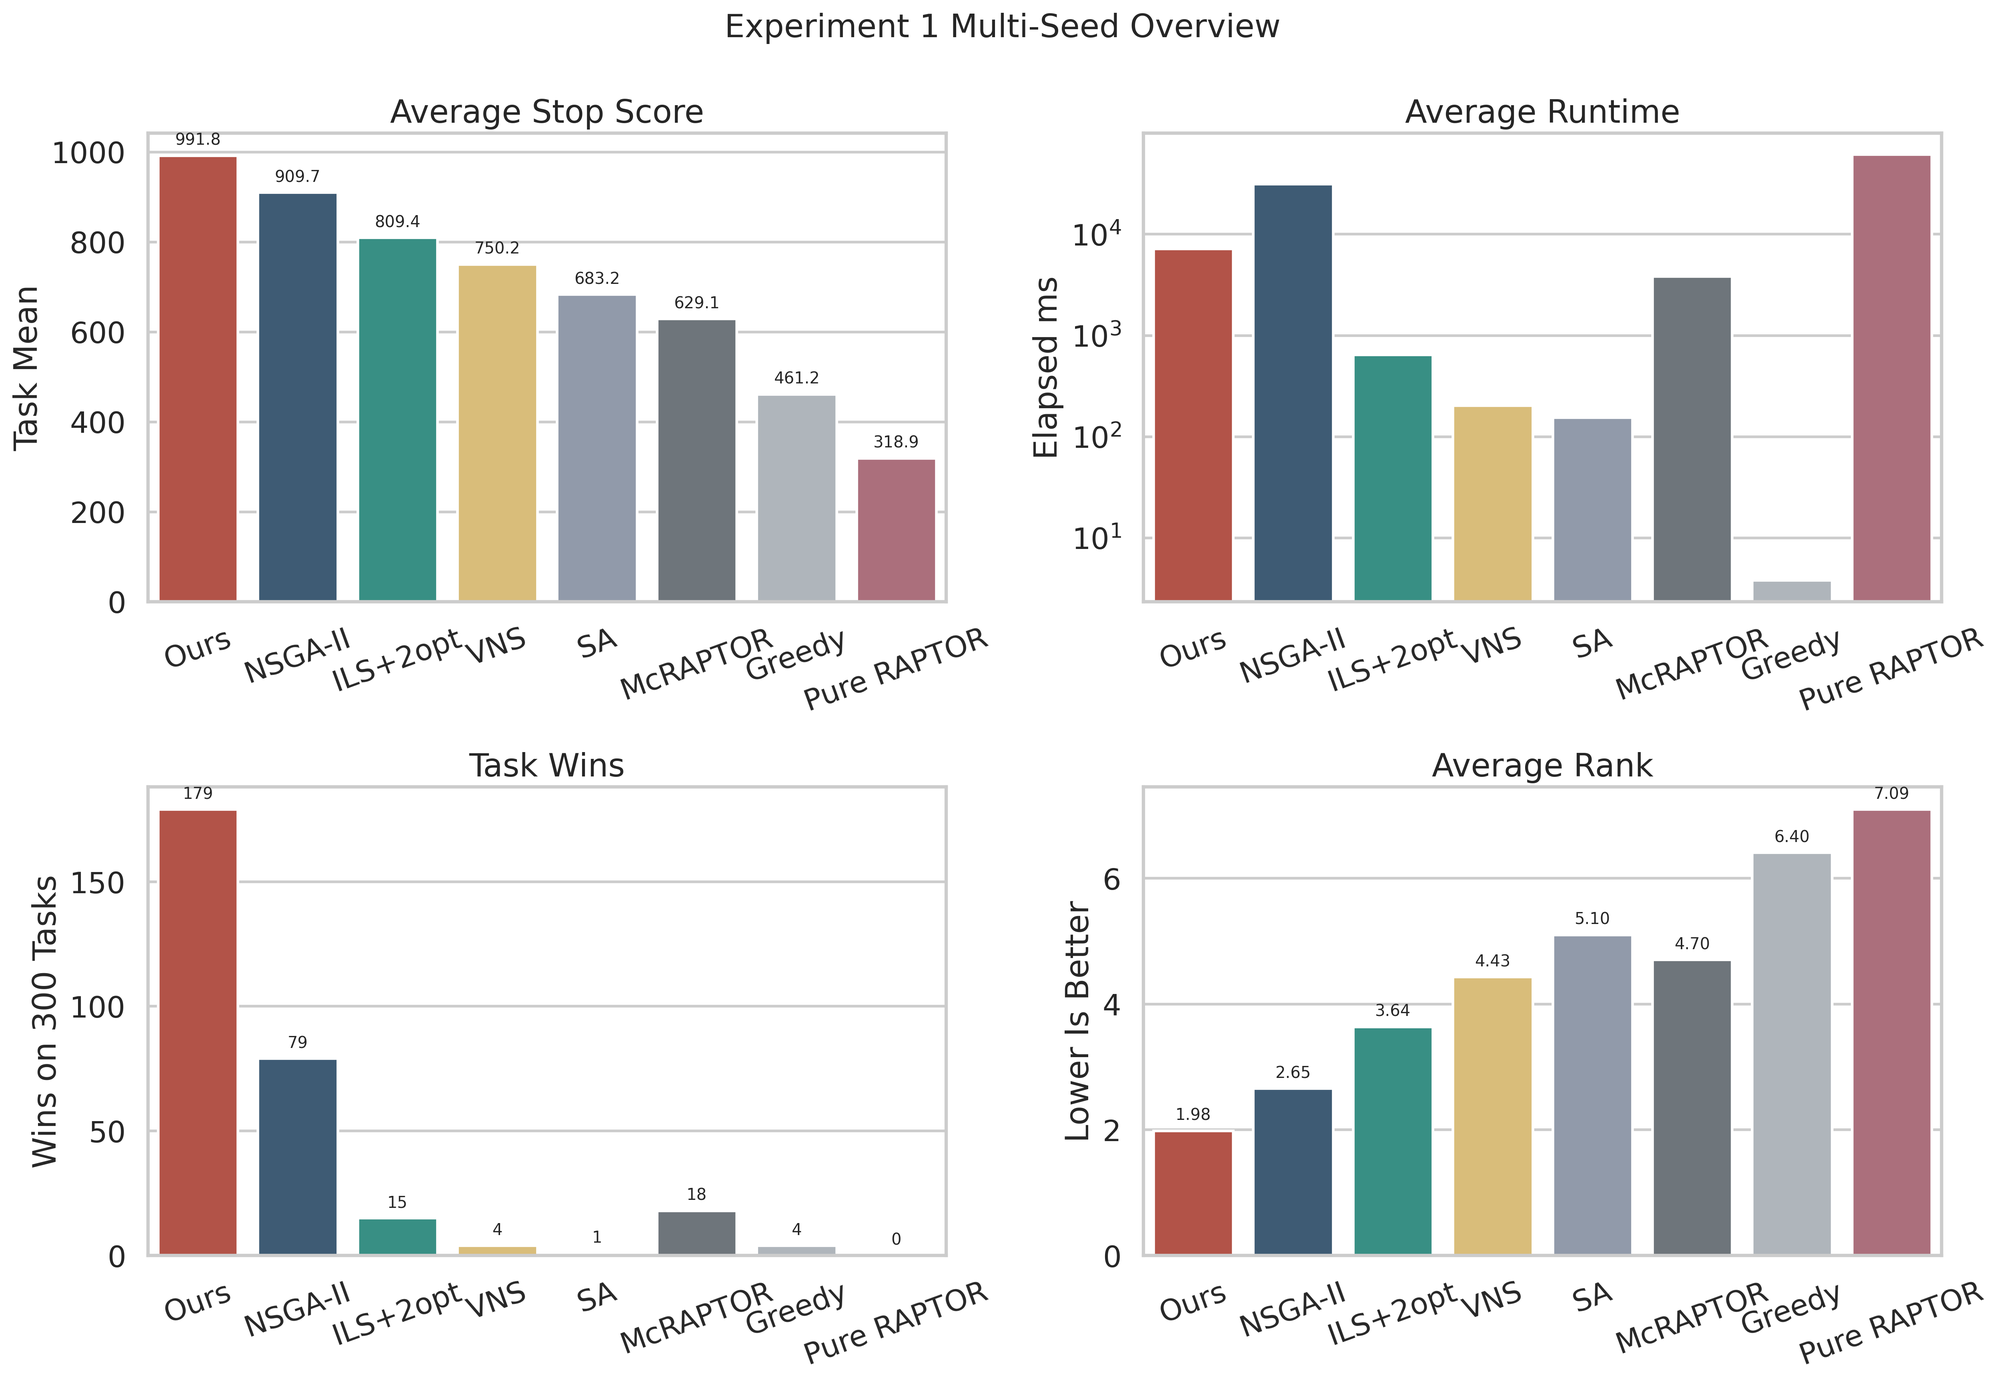
\includegraphics[width=0.93\linewidth]{figures/exp1/exp1_score_guided_multiseed_overview_20260403.png}
    \caption{実験1の全体 overview．平均 stop score，runtime，task wins，average rank をまとめて示している}
\end{figure}

\begin{figure}[H]
    \centering
    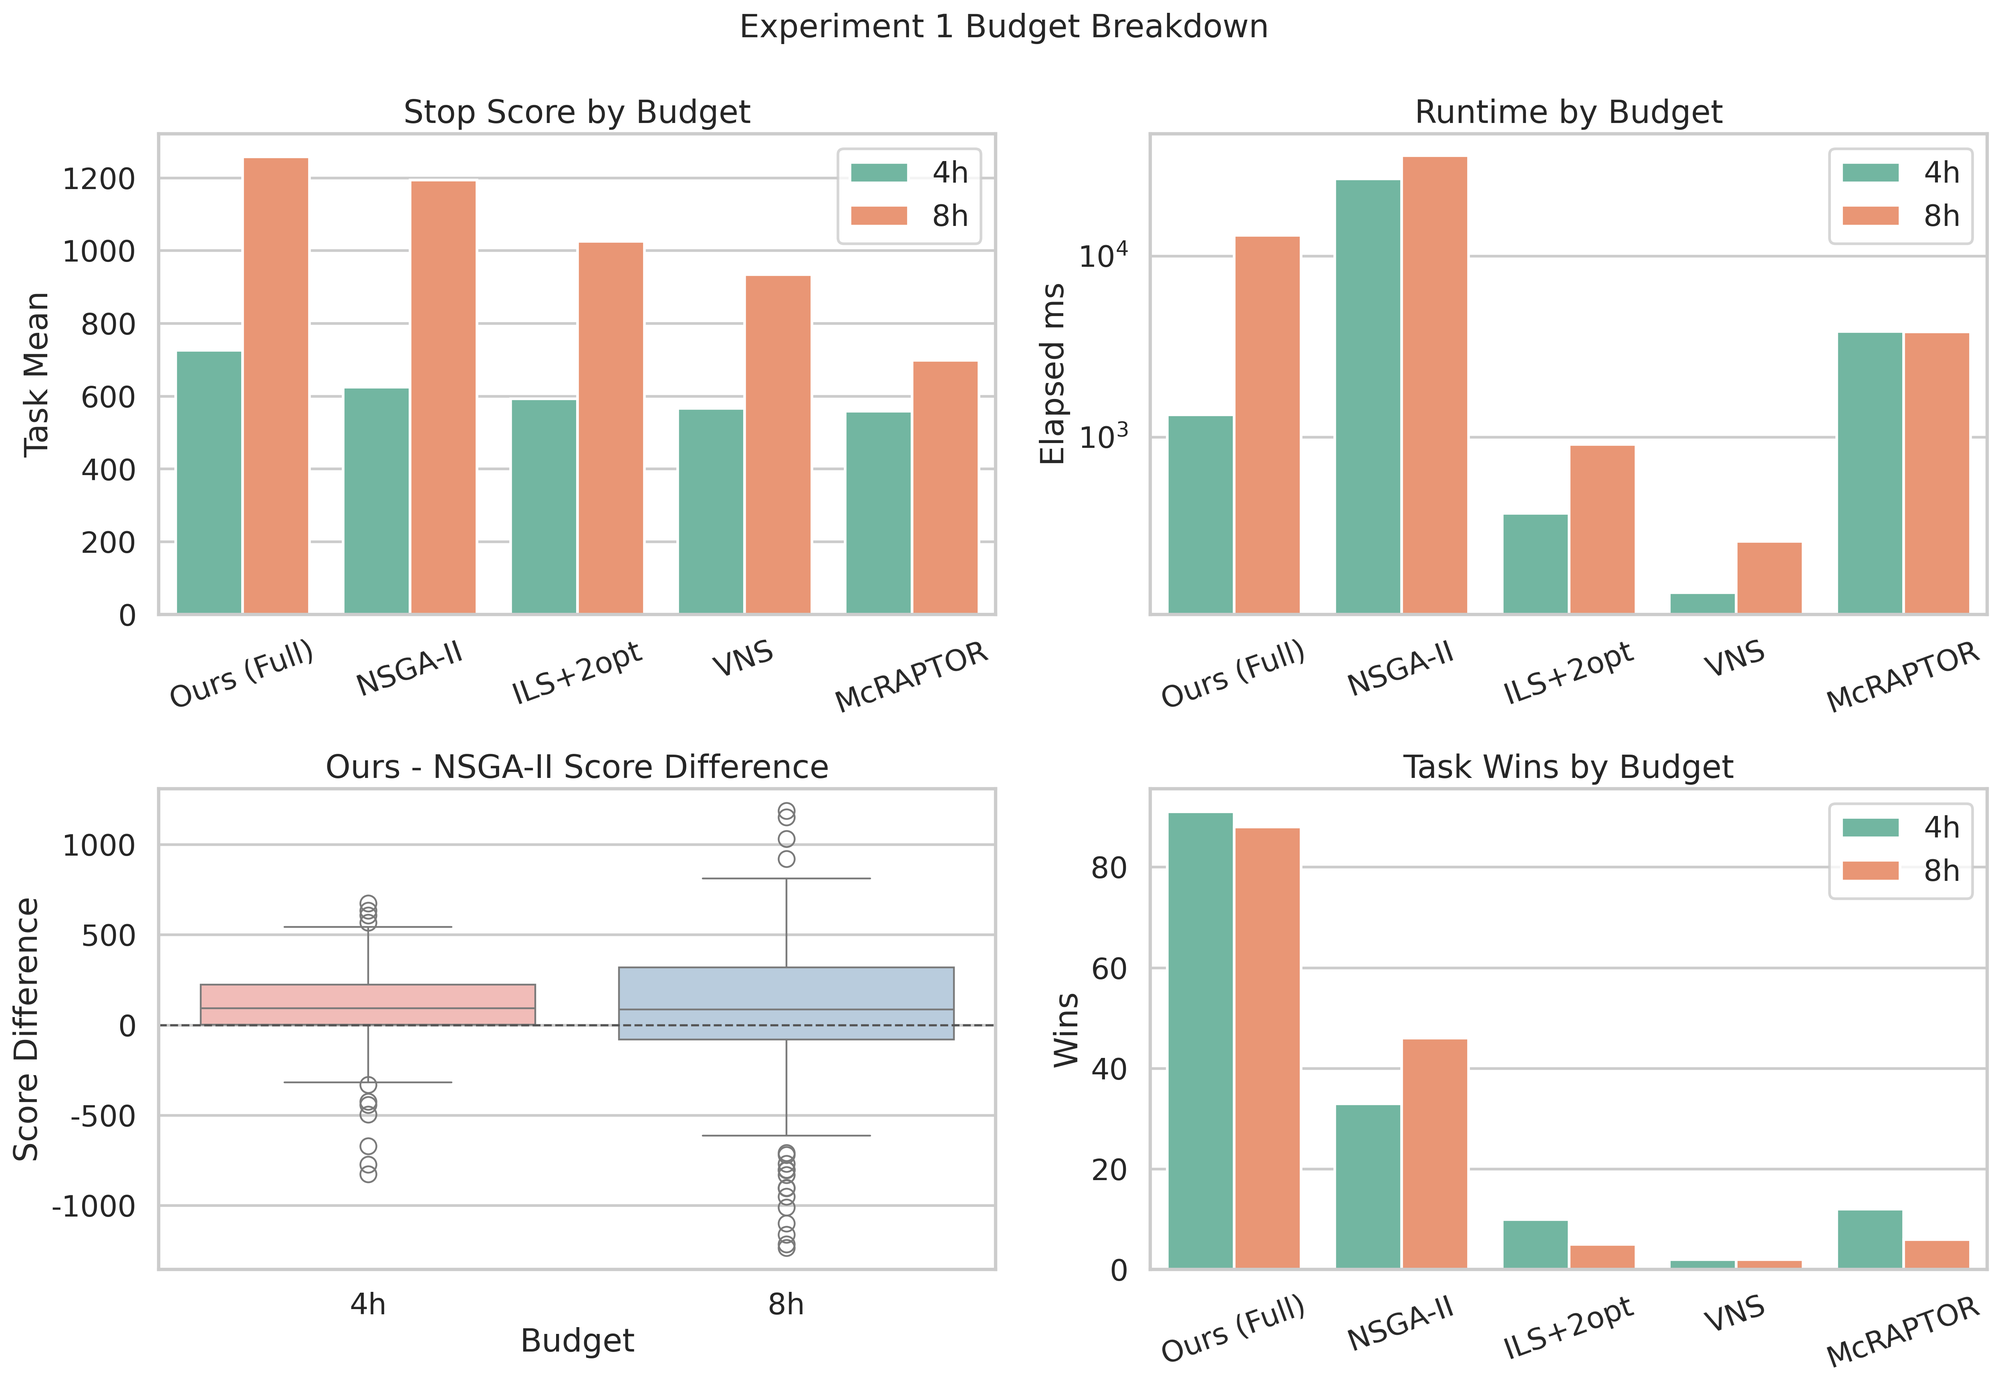
\includegraphics[width=0.93\linewidth]{figures/exp1/exp1_score_guided_multiseed_budget_20260403.png}
    \caption{実験1の budget 別比較．4h / 8h の両方で Ours が高 score 側にいることを確認できる}
\end{figure}

\subsection*{結果の解釈}
この実験から言えそうなのは，
単に「Ours が平均 1 位」ということだけではなく，
\textbf{NSGA-II よりかなり短い時間で，しかもより高い score を返す query が多い}
という点です．
特に 4h では Ours が 30 query 中 27 query で
「score でも勝ち，時間でも勝つ」形になっており，
主張として非常にわかりやすいです．
8h では差が少し複雑になりますが，
それでも overall の平均では Ours が score と runtime の両方で有利です．

また，score seed を変えても Ours - NSGA-II の平均差が常に正だったので，
「たまたまある score map だけで Ours に都合がよかった」
という読み方はしにくいと思っています．

\subsection*{先生にご意見をいただきたい点}
\begin{itemize}
    \item 実験1では「平均 score 1 位」よりも，「高 score かつ高速な query が多い」点を主張の中心に置く方がよいでしょうか．
    \item 現在の図では overview と budget breakdown の 2 枚を使う想定ですが，先生に見ていただく版では 2 枚とも入れた方が理解しやすいか，あるいは 1 枚に絞るべきか，ご意見をいただきたいです．
\end{itemize}

\clearpage
\section{実験2：三層 pruning の ablation}
\subsection*{目的}
実験2の目的は，
Full system が良いということを示すだけでなく，
Beam，Dominance，Negative の三層が
それぞれ何に効いているかを切り分けて説明することです．
ここでは特に，
\textbf{(1) Dominance は本当に必須か}，
\textbf{(2) Beam はどの budget 条件で効くか}，
\textbf{(3) Negative は score 向上ではなく theme 整合性のための層なのか}
を確認したいと考えました．

\subsection*{実験設定}
主アブレーションは，score-guided 主タスクに対して
次の 7 variants を比較しています．
\begin{itemize}
    \item Ours (Full)
    \item Ours (NoNeg)
    \item Ours (NoDom)
    \item Ours (NoBeam)
    \item Ours (NoDom-NoNeg)
    \item Ours (NoBeam-NoNeg)
    \item Ours (NoBeam-NoDom-NoNeg)
\end{itemize}

主アブレーションの集計単位は
\((origin,\ depart\_time,\ budget,\ score\_seed)\)
です．
さらに Negative の役割を詳しく見るために，
theme-oriented supporting task も別に用意し，
Full と NoNeg を同じ paired case 上で比較しました．
この supporting task では 384 paired cases を見ています．

\subsection*{評価指標}
主アブレーションでは次の指標を使っています．
\begin{itemize}
    \item \texttt{stop\_score\_total}
    \item \texttt{elapsed\_ms}
    \item \texttt{labels}
    \item \texttt{cap\_hit\_rate}
    \item \texttt{success\_rate}
\end{itemize}

ここで \texttt{labels} は探索中に保持した状態数の近似であり，
探索空間やメモリ負荷の大きさを見るために使っています．
\texttt{cap\_hit\_rate} は safety cap に達した割合で，
探索が制御不能になりかけていないかを見る指標です．

Negative の supporting task ではこれに加えて，
\texttt{theme\_hit\_ratio} と
\texttt{theme\_satisfied\_rate} を見ています．
\texttt{theme\_hit\_ratio} は route の中で対象 theme に合う要素がどの程度維持されたか，
\texttt{theme\_satisfied\_rate} はその比率が threshold を満たした割合として読んでいます．

\subsection*{主要結果}
主アブレーション全体を見ると，
Full は 999.27 点，4668.15 ms，labels 115437 で，
最もバランスがよい位置にあります．
NoNeg はほぼ同点ですが，
NoDom は quality・runtime・labels のすべてが悪化します．
NoBeam はさらに極端で，
score も落ち，runtime と labels が大きく膨らみます．

\begin{table}[H]
    \centering
    \small
    \caption{実験2の主 ablation 結果}
    \resizebox{\linewidth}{!}{%
    \begin{tabular}{lrrrrr}
        \toprule
        Variant & Stop score & Runtime (ms) & Labels & Success (\%) & Cap hit (\%) \\
        \midrule
        Ours (Full) & 999.27 & 4668.15 & 115437 & 97.78 & 0.00 \\
        Ours (NoNeg) & 996.10 & 4865.37 & 119327 & 97.22 & 0.00 \\
        Ours (NoDom) & 971.91 & 13589.45 & 349946 & 97.78 & 0.00 \\
        Ours (NoBeam) & 912.04 & 44486.93 & 1487640 & 97.78 & 59.44 \\
        Ours (NoDom-NoNeg) & 973.06 & 12984.17 & 350981 & 97.78 & 0.00 \\
        Ours (NoBeam-NoNeg) & 911.56 & 44700.47 & 1509040 & 97.78 & 60.00 \\
        Ours (NoBeam-NoDom-NoNeg) & 289.37 & 20929.99 & 1000000 & 100.00 & 100.00 \\
        \bottomrule
    \end{tabular}}
\end{table}

Beam の役割は budget によってかなり違います．
4h では NoBeam が Full より少し高い score を出すことがありますが，
その代償として runtime は約 35 倍に増え，
cap hit も 18.89\% まで上がります．
8h では NoBeam の score 自体も落ち，
cap hit は 100\% になります．
したがって Beam は「常に quality を上げる層」というより，
長時間 budget で探索を壊さないための stabilizer と読むのが自然だと思っています．

\begin{table}[H]
    \centering
    \small
    \caption{Beam の役割を見るための Full vs NoBeam 比較}
    \begin{tabular}{lrrrrr}
        \toprule
        Budget & Variant & Stop score & Runtime (ms) & Labels & Cap hit (\%) \\
        \midrule
        4h & Full & 737.04 & 771.47 & 24.4K & 0.00 \\
        4h & NoBeam & 803.80 & 27076.50 & 847.1K & 18.89 \\
        8h & Full & 1261.50 & 8564.82 & 206.5K & 0.00 \\
        8h & NoBeam & 1020.28 & 61897.36 & 2.13M & 100.00 \\
        \bottomrule
    \end{tabular}
\end{table}

Negative の supporting task では，
Full は NoNeg より theme 整合性をかなり強く維持しています．
平均では，
ThemeHit が 0.965 vs 0.677，
ThemeSat が 0.958 vs 0.646 であり，
paired comparison でも 384 case 中 226 case で Full が theme-hit を改善しました．
しかも最終 route は 384 case 中 366 case で実際に変わっているので，
Negative は単に search trace を少し変えているだけではなく，
出力 route そのものの選び方を変えていると読めます．

\begin{table}[H]
    \centering
    \small
    \caption{Negative supporting task における Full vs NoNeg}
    \begin{tabular}{lrrrrr}
        \toprule
        Variant & Ride min & ThemeHit & ThemeSat & Runtime (ms) & Labels \\
        \midrule
        Ours (Full) & 318.98 & 0.965 & 0.958 & 18473.95 & 264348.8 \\
        Ours (NoNeg) & 281.09 & 0.677 & 0.646 & 6304.29 & 104760.0 \\
        \bottomrule
    \end{tabular}
\end{table}

\begin{table}[H]
    \centering
    \small
    \caption{Negative supporting task の paired 差分要約}
    \begin{tabular}{lrrrr}
        \toprule
        指標 & Mean delta (Full - NoNeg) & Full better & Tie & NoNeg better \\
        \midrule
        ThemeHit & +0.2882 & 226 & 156 & 2 \\
        ThemeSat & +0.3125 & 120 & 264 & 0 \\
        RideMinutes & +37.891 & 210 & 28 & 146 \\
        Runtime (ms) & +12169.664 & 8 & 0 & 376 \\
        \bottomrule
    \end{tabular}
\end{table}

\begin{figure}[H]
    \centering
    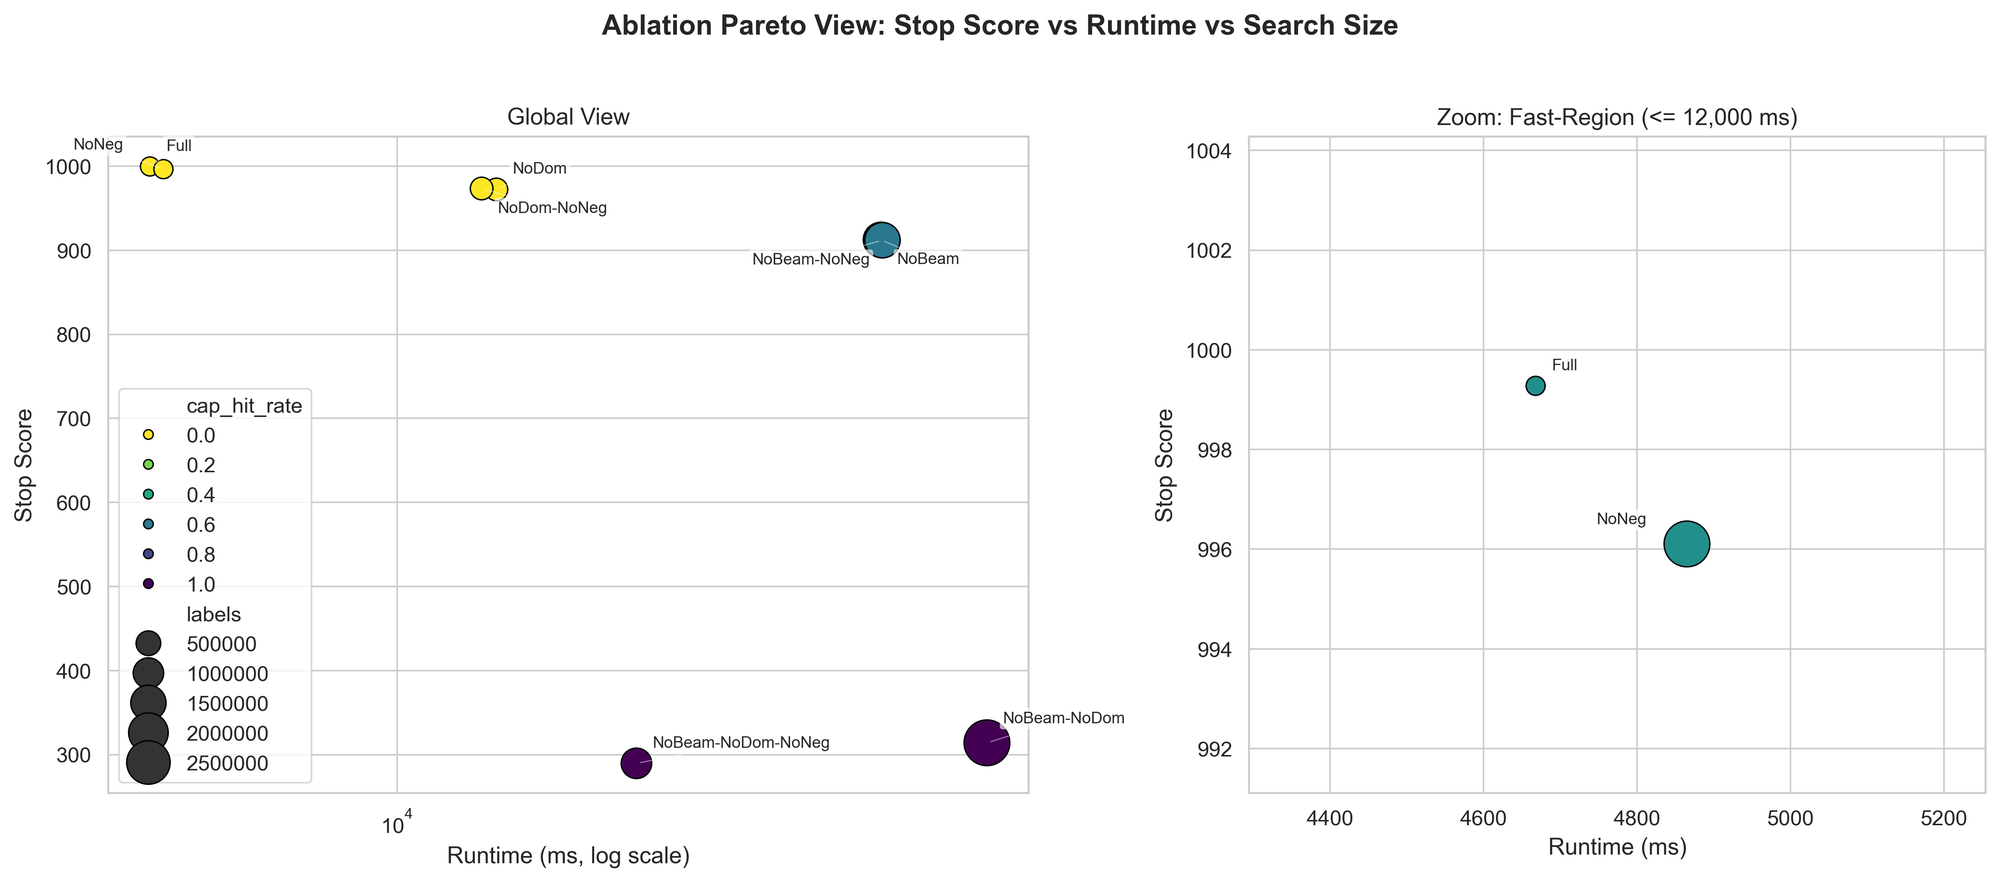
\includegraphics[width=0.95\linewidth]{figures/exp2/exp2_ablation_pareto_scatter.png}
    \caption{主 ablation の Pareto view．Full が score，runtime，search size の 3 軸で最も説明しやすい位置にある}
\end{figure}

\begin{figure}[H]
    \centering
    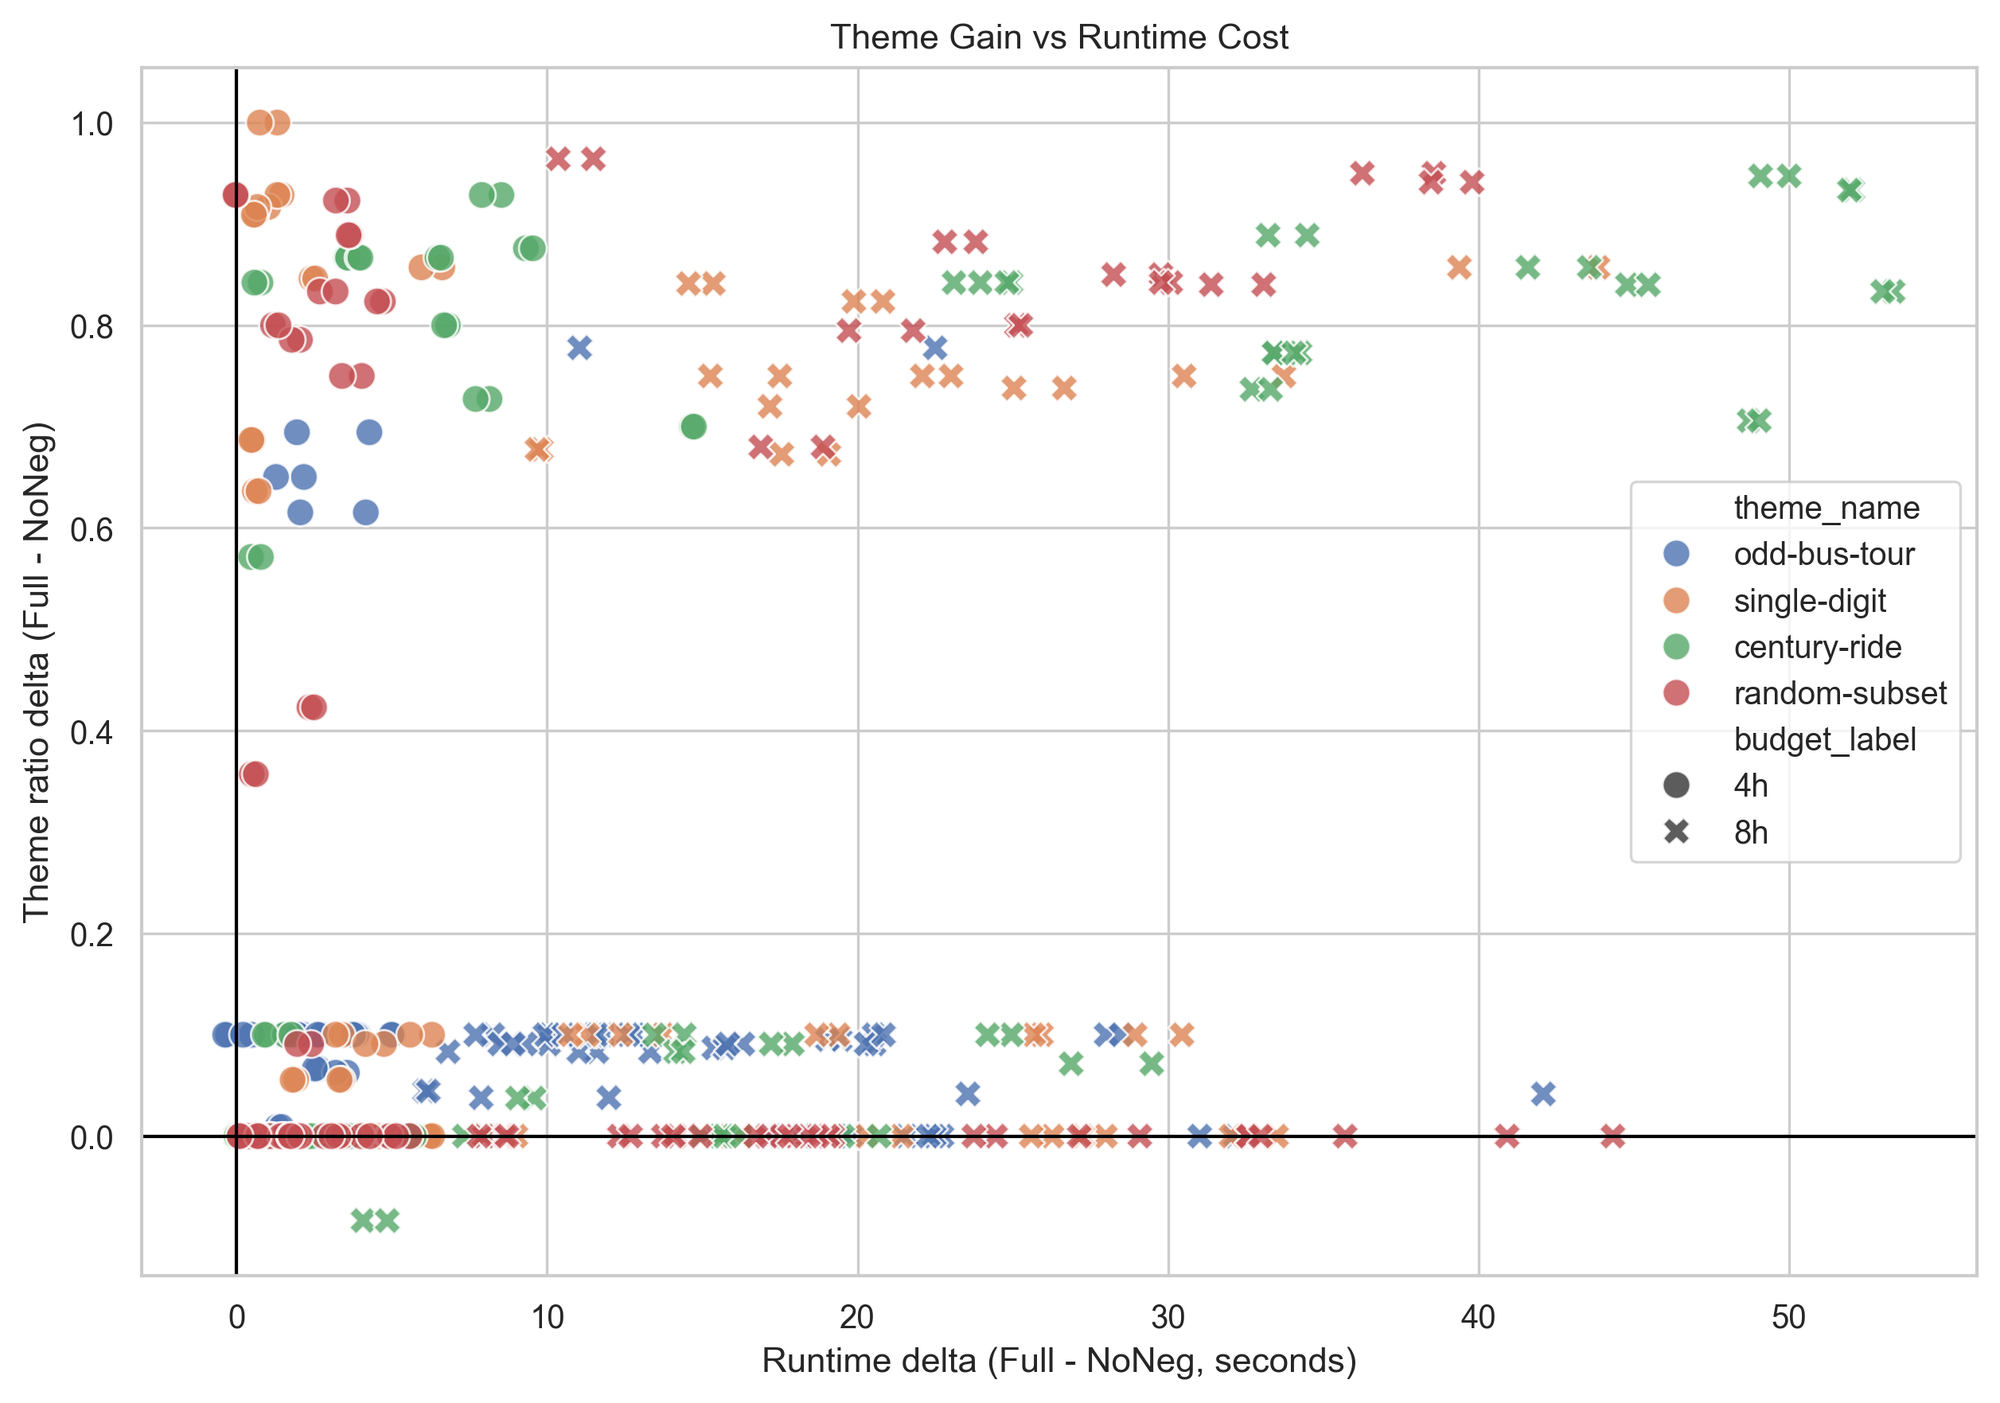
\includegraphics[width=0.92\linewidth]{figures/exp2/exp2_supporting_negative_tradeoff.png}
    \caption{Negative supporting task．runtime 増加の代わりに theme-hit が改善する case が多いことを示している}
\end{figure}

\subsection*{結果の解釈}
この実験をまとめると，
\textbf{Dominance は必須の計算可能性レイヤー}，
\textbf{Beam は高 budget 条件での安定化レイヤー}，
\textbf{Negative は theme-oriented route を崩さないための制約整合性レイヤー}
として説明するのが最も自然です．

特に Dominance は，外したとたんに score も runtime も labels も悪化するので，
三層の中でも中核寄りの役割として書けそうです．
一方で Negative は，
score-guided 主タスクだけを見ると差が小さく見えますが，
theme-oriented supporting task を見ると
「何のための layer なのか」が明確になります．

\subsection*{先生にご意見をいただきたい点}
\begin{itemize}
    \item 実験2では Dominance を中核貢献として強く押し，Beam と Negative は役割分担として整理する書き方でよいか．
    \item Negative は main benchmark ではなく supporting task の中で主張する方が正確だと思っていますが，この配置で問題ないかご意見をいただきたいです．
\end{itemize}

\clearpage
\section{実験3：quality-speed balance の整理}
\subsection*{目的}
実験3の目的は，
実験1の結果を
「平均 score が高い」という 1 軸だけでなく，
quality と runtime のバランスとしても説明できるかを整理することです．
ここで確認したいのは，
\reraptor{} が
\textbf{常に最高 score の手法であるか}ではなく，
\textbf{高い score と現実的な runtime の両方を考えると frontier の近くに最も安定して位置するか}
という点です．

\subsection*{実験設定}
この実験は，実験1の source results を使って後段分析を行ったものです．
したがって対象 task は実験1と同じで，
10 origins，
3 departure times，
2 budgets，
5 score seeds の組合せです．
task-level では 300 rows，
query-level では 60 rows を使っています．

\subsection*{評価指標}
ここでは主に次の 3 つを見ています．
\begin{itemize}
    \item \texttt{pareto\_front\_rate}：同一 task 内で，score と runtime の 2 軸において Pareto front に乗る頻度
    \item \texttt{avg\_ideal\_distance}：正規化した「高 score・低 runtime」の理想点にどれだけ近いか
    \item \texttt{tradeoff\_category}：Ours と NSGA-II を比べたとき，「高 score + 高速」なのか，「低 score だが高速」なのかを分類したもの
\end{itemize}

\texttt{pareto\_front\_rate} だけを見ると，
Greedy のように極端に速い手法も front に残りやすいので，
論文の説明には \texttt{avg\_ideal\_distance} を併用するのが重要だと考えています．

\subsection*{主要結果}
task-level summary では，
Ours が Pareto front rate 0.800，
ideal-point distance 0.222 で最良でした．
query-level でも Ours の ideal-point distance は 0.170 で最良です．
したがって，少なくとも現在の主タスクでは，
Ours が quality-speed frontier の近くに最も安定していると読めます．

\begin{table}[H]
    \centering
    \small
    \caption{実験3の quality-speed balance 要約（task-level）}
    \resizebox{\linewidth}{!}{%
    \begin{tabular}{lrrrrr}
        \toprule
        Algorithm & Avg stop score & Avg runtime (ms) & Score / hour & Pareto front rate & Ideal distance \\
        \midrule
        Ours (Full) & 991.83 & 7175.91 & 188.06 & 0.800 & 0.222 \\
        ILS+2opt & 809.45 & 645.49 & 145.40 & 0.647 & 0.367 \\
        VNS & 750.23 & 202.28 & 136.71 & 0.693 & 0.433 \\
        SA & 683.22 & 153.73 & 124.92 & 0.700 & 0.518 \\
        McRAPTOR & 629.05 & 3825.95 & 146.42 & 0.127 & 0.506 \\
        NSGA-II & 909.70 & 31198.10 & 167.90 & 0.283 & 0.625 \\
        Greedy (L=3) & 461.19 & 3.79 & 86.15 & 1.000 & 0.749 \\
        Pure RAPTOR & 318.91 & 61287.02 & 185.14 & 0.000 & 1.349 \\
        \bottomrule
    \end{tabular}}
\end{table}

Ours vs NSGA-II を直接比べると，
task-level 300 task のうち
199 task で Ours が
「higher score + faster」でした．
query-level でも 60 query 中 46 query で同じ関係が成り立っています．
4h では 30 query 中 27 query で Ours が
「higher score + faster」でしたが，
8h では 30 query 中 19 query でそうなっており，
残り 11 query では
「NSGA-II の方が高 score だが，Ours の方が速い」
という関係でした．

\begin{table}[H]
    \centering
    \small
    \caption{実験3の Ours vs NSGA-II 比較（query-level）}
    \begin{tabular}{lrrr}
        \toprule
        Budget / 集計 & Higher score + faster & Lower score + faster & Share of higher score + faster \\
        \midrule
        4h (30 queries) & 27 & 3 & 0.900 \\
        8h (30 queries) & 19 & 11 & 0.633 \\
        Overall (60 queries) & 46 & 14 & 0.767 \\
        \bottomrule
    \end{tabular}
\end{table}

\begin{figure}[H]
    \centering
    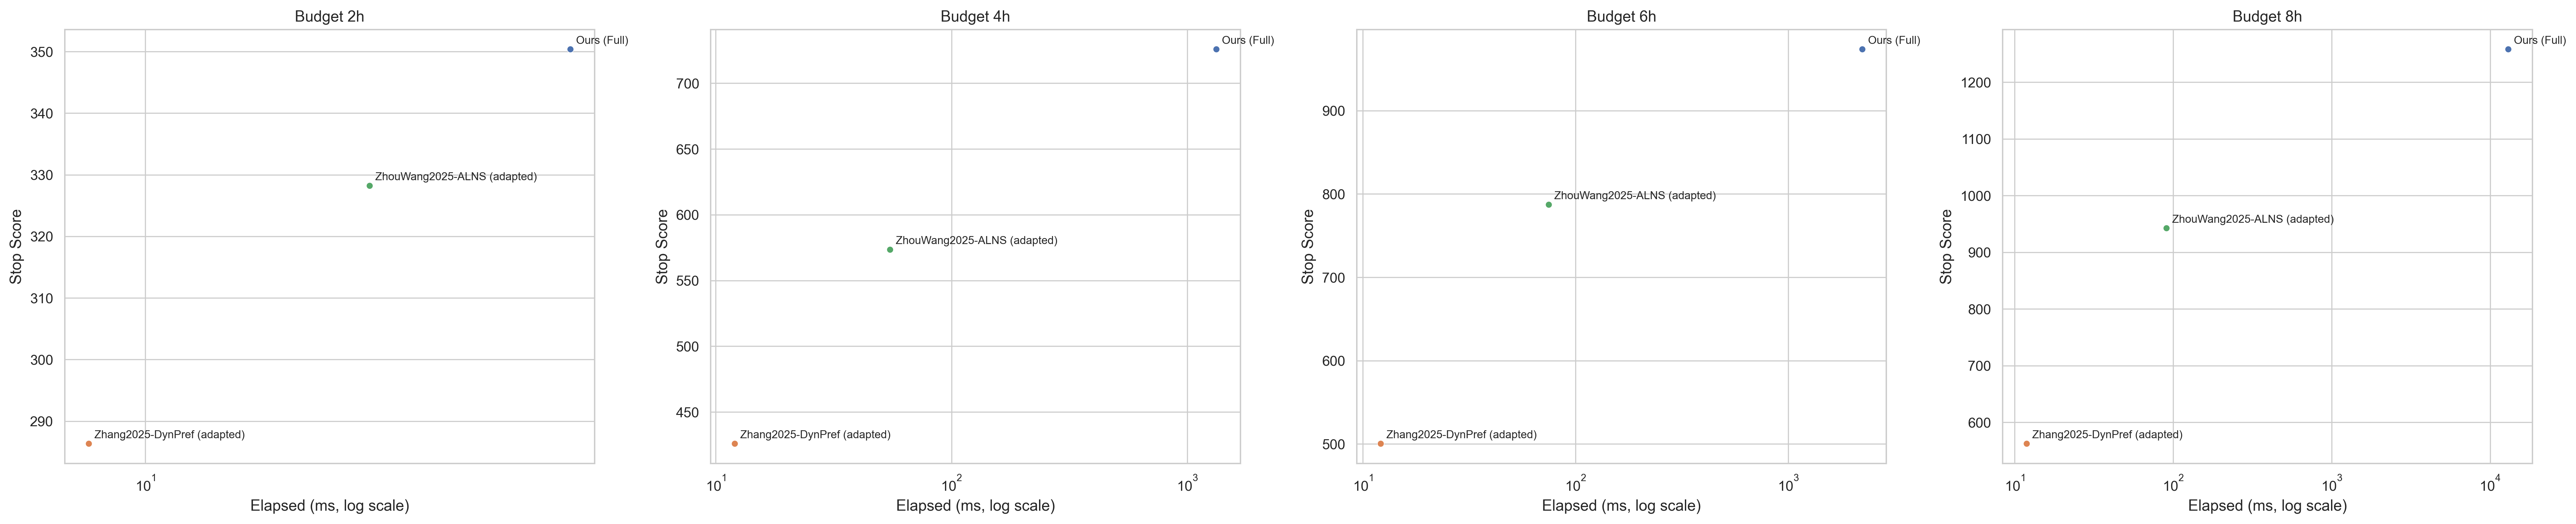
\includegraphics[width=0.95\linewidth]{figures/exp3/exp3_quality_speed_scatter.png}
    \caption{実験3の quality-speed scatter．Ours は高 score 側に位置しつつ，NSGA-II より左側，つまり短い runtime 側にある}
\end{figure}

\begin{figure}[H]
    \centering
    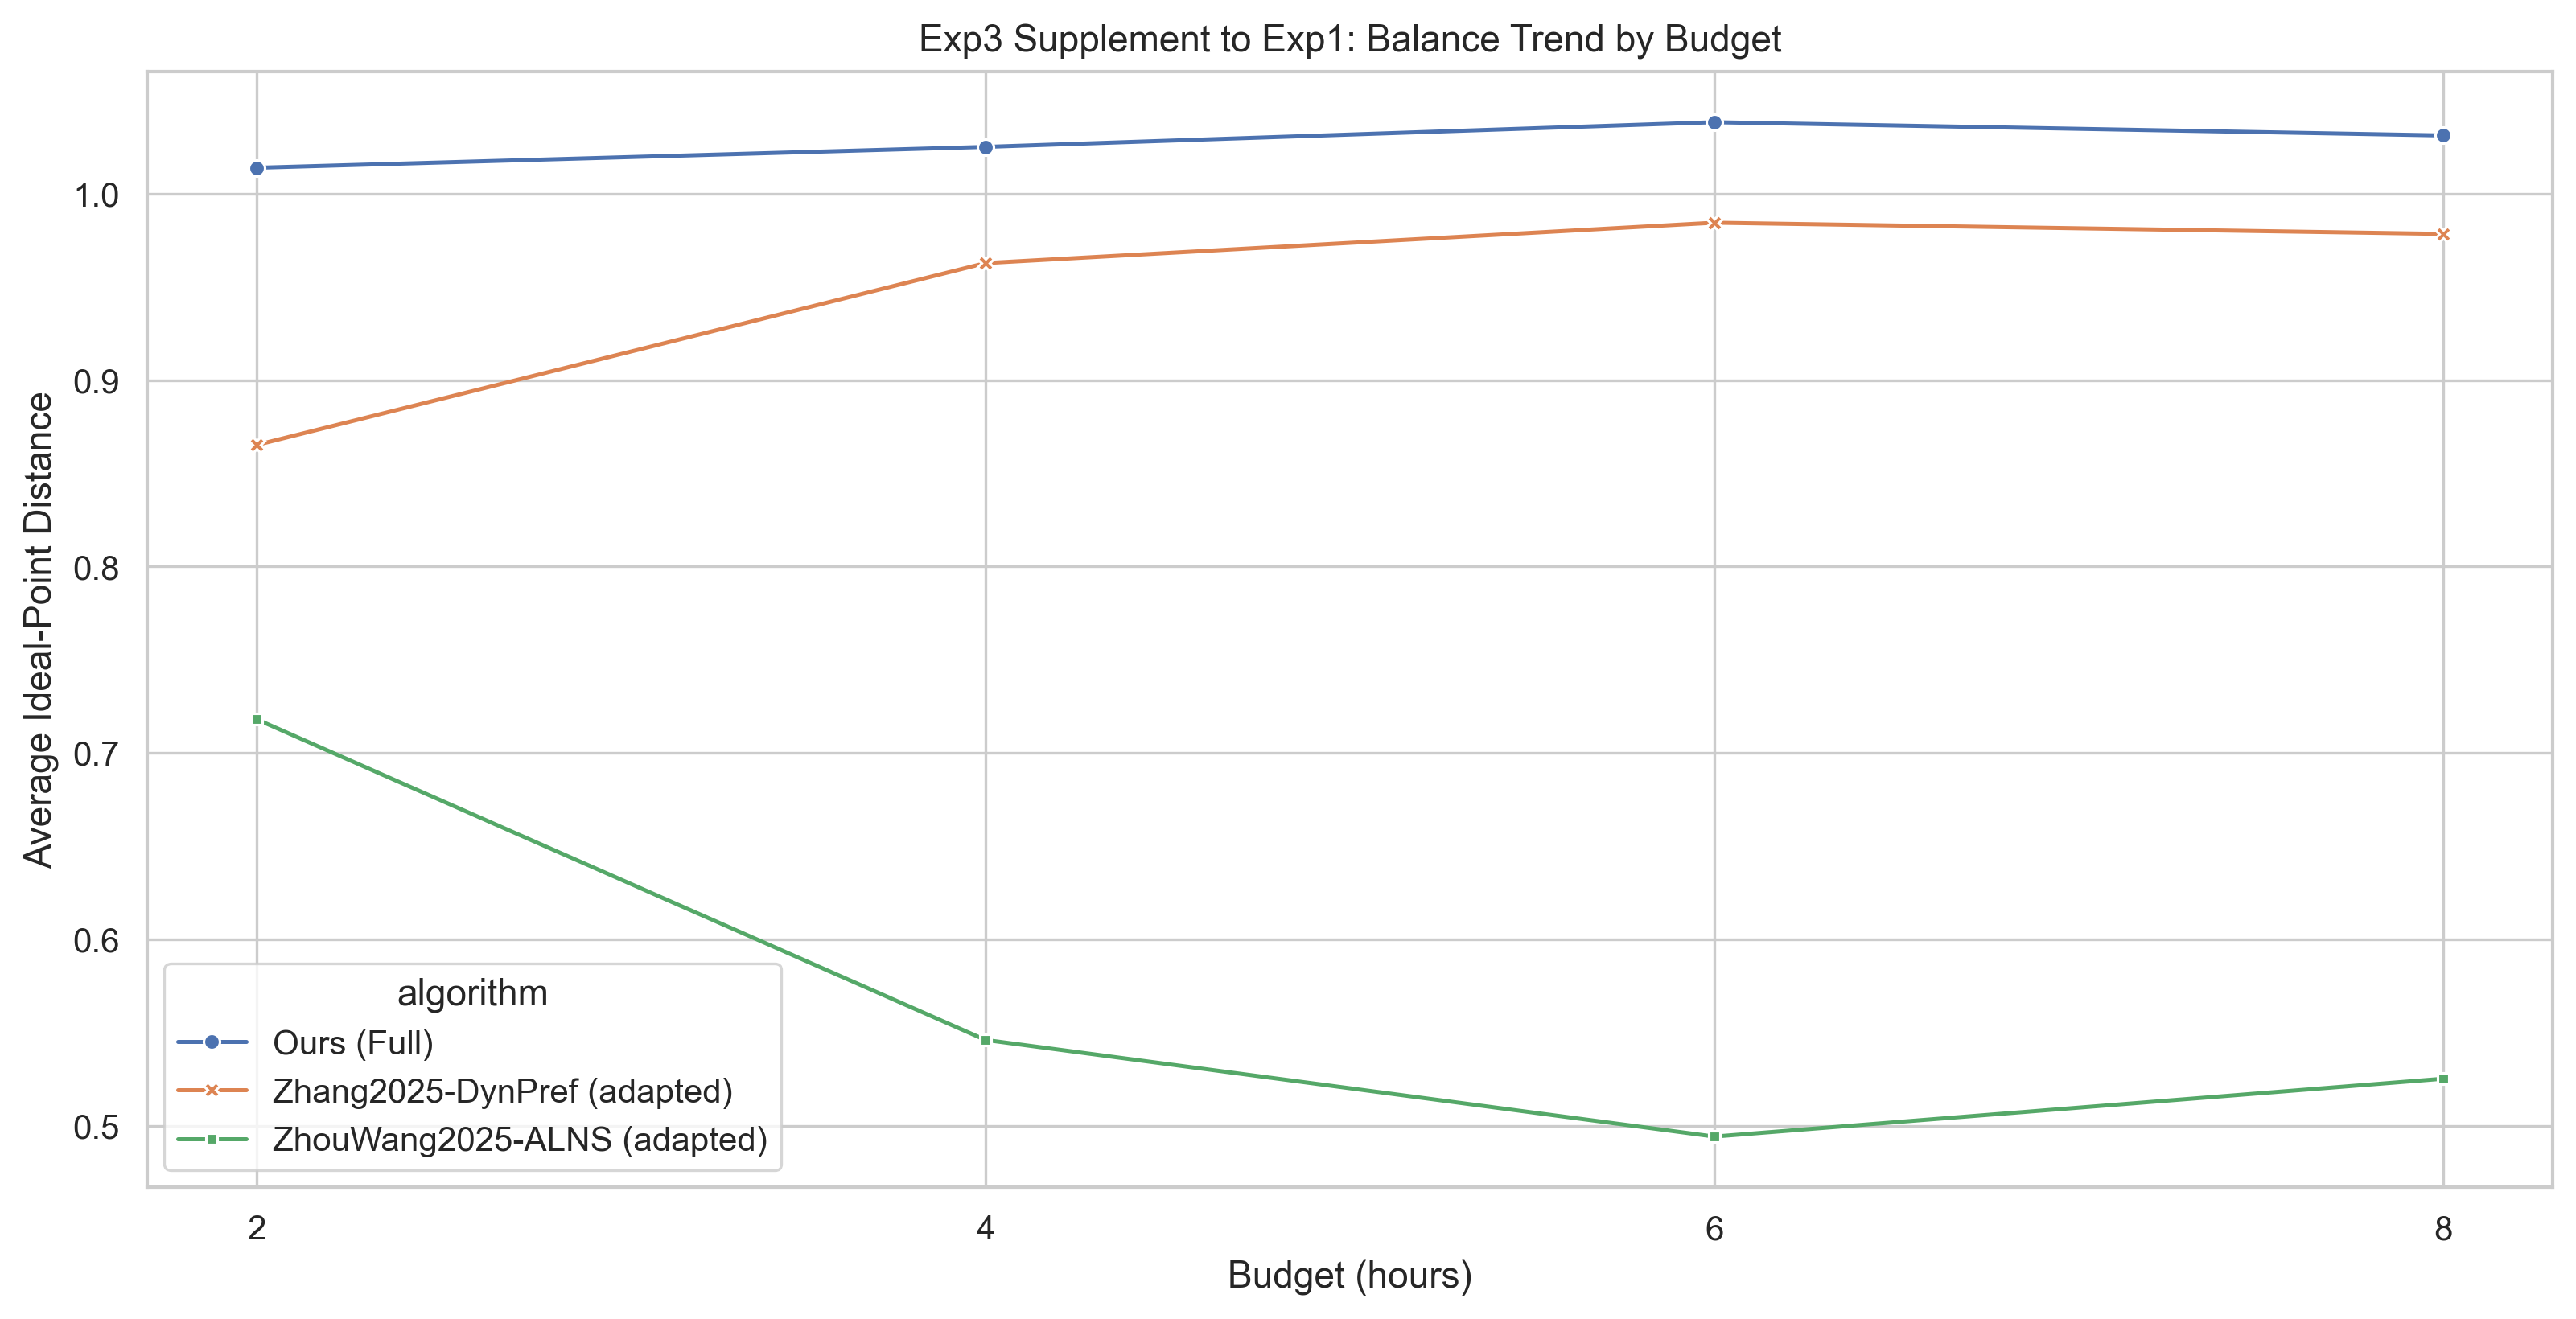
\includegraphics[width=0.92\linewidth]{figures/exp3/exp3_ideal_distance.png}
    \caption{実験3の average ideal-point distance．Greedy のように Pareto front に頻繁に残る手法でも，理想点からの距離では Ours に及ばないことがわかる}
\end{figure}

\subsection*{結果の解釈}
この実験で大事なのは，
「Ours が every query で universal best」と言いたいわけではない点です．
実際，8h では NSGA-II の方が高い score に到達する query もあります．
しかし，その場合でも NSGA-II は runtime がかなり長くなりやすく，
全体として見ると Ours の方が
高 score と現実的 runtime の両方を満たす位置に安定しています．

したがって，
論文上の主張としては
\textbf{overall quality-speed balance} を中心に置き，
Exp1 の benchmark 結果と組み合わせて
「なぜ Ours を main method として推したいのか」
を説明するのがよいと思っています．

\subsection*{先生にご意見をいただきたい点}
\begin{itemize}
    \item 実験3は，実験1の補強として「balance analysis」に位置づけるのがよいか，あるいは独立の主要実験として残すべきか，ご意見をいただきたいです．
    \item 指標としては \texttt{pareto\_front\_rate} と \texttt{ideal\_distance} の両方を出していますが，先生にお見せする版では \texttt{ideal\_distance} を中心に読んでもらう方がわかりやすいか確認したいです．
\end{itemize}

\clearpage
\section{実験4：route case study}
\subsection*{目的}
現在の実験4は，旧版の scenario generalization ではなく，
score-guided 主タスクで得られた差を
具体的な route の形として読みやすくするための qualitative case study です．
したがって，この実験の目的は
「さらに benchmark を 1 本足す」ことではなく，
\textbf{実験1・3の定量差が，route の構造としてどう見えるかを説明すること}
にあります．

\subsection*{case の選び方}
今回使っている case は，実験1・3の結果から次の 3 つを選んでいます．
\begin{itemize}
    \item Case A：Ours が score と runtime の両方で明確に勝っている成功例
    \item Case B：Ours が top score ではないが，quality-speed balance では最も説明しやすい例
    \item Case C：Ours が速い一方で最高 score は逃している反例
\end{itemize}

各 panel には，
stop score，
generation time，
score per hour，
scored stops が併記されているので，
「高い score を出している route は，本当に route の広がりや stop の取り方でも違って見えるか」
を直感的に確認できます．

\subsection*{主要結果}

\begin{table}[H]
    \centering
    \small
    \caption{実験4で使う 3 case の要約}
    \begin{tabularx}{\linewidth}{L{1.3cm}L{4.4cm}X}
        \toprule
        Case & Query & 何を見せたいか \\
        \midrule
        A & fukudaimae / 07:00 / 8h / score\_seed=20260325 & Ours が 1459.0 / 9091.1 ms で，NSGA-II の 854.0 / 14129.0 ms を両方上回る典型的成功例 \\
        B & tenjin / 07:00 / 8h / score\_seed=20260325 & Ours は top score ではないが，1276.0 / 4473.7 ms で，NSGA-II の高 score と SA の超高速の中間に位置する balance 例 \\
        C & yakuin / 14:00 / 8h / score\_seed=20260327 & Ours は 1358.0 / 2730.8 ms で速いが，NSGA-II の 1556.0 には届かない．universal dominance を主張しないための反例 \\
        \bottomrule
    \end{tabularx}
\end{table}

\begin{table}[H]
    \centering
    \small
    \caption{Case A / B / C の数値比較}
    \resizebox{\linewidth}{!}{%
    \begin{tabular}{llrrrr}
        \toprule
        Case & Algorithm & Stop score & Gen time (ms) & Score / hour & Scored stops \\
        \midrule
        A & Ours & 1459.0 & 9091.1 & 185.5 & 22 \\
        A & NSGA-II & 854.0 & 14129.0 & 108.1 & 13 \\
        A & VNS & 508.0 & 37.0 & 68.5 & 10 \\
        \midrule
        B & Ours & 1276.0 & 4473.7 & 164.6 & 18 \\
        B & NSGA-II & 1590.0 & 18956.2 & 200.8 & 22 \\
        B & SA & 1506.0 & 156.4 & 192.7 & 20 \\
        \midrule
        C & Ours & 1358.0 & 2730.8 & 187.3 & 18 \\
        C & NSGA-II & 1556.0 & 20367.1 & 207.9 & 19 \\
        C & VNS & 1461.0 & 192.6 & 186.5 & 19 \\
        \bottomrule
    \end{tabular}}
\end{table}

\begin{figure}[H]
    \centering
    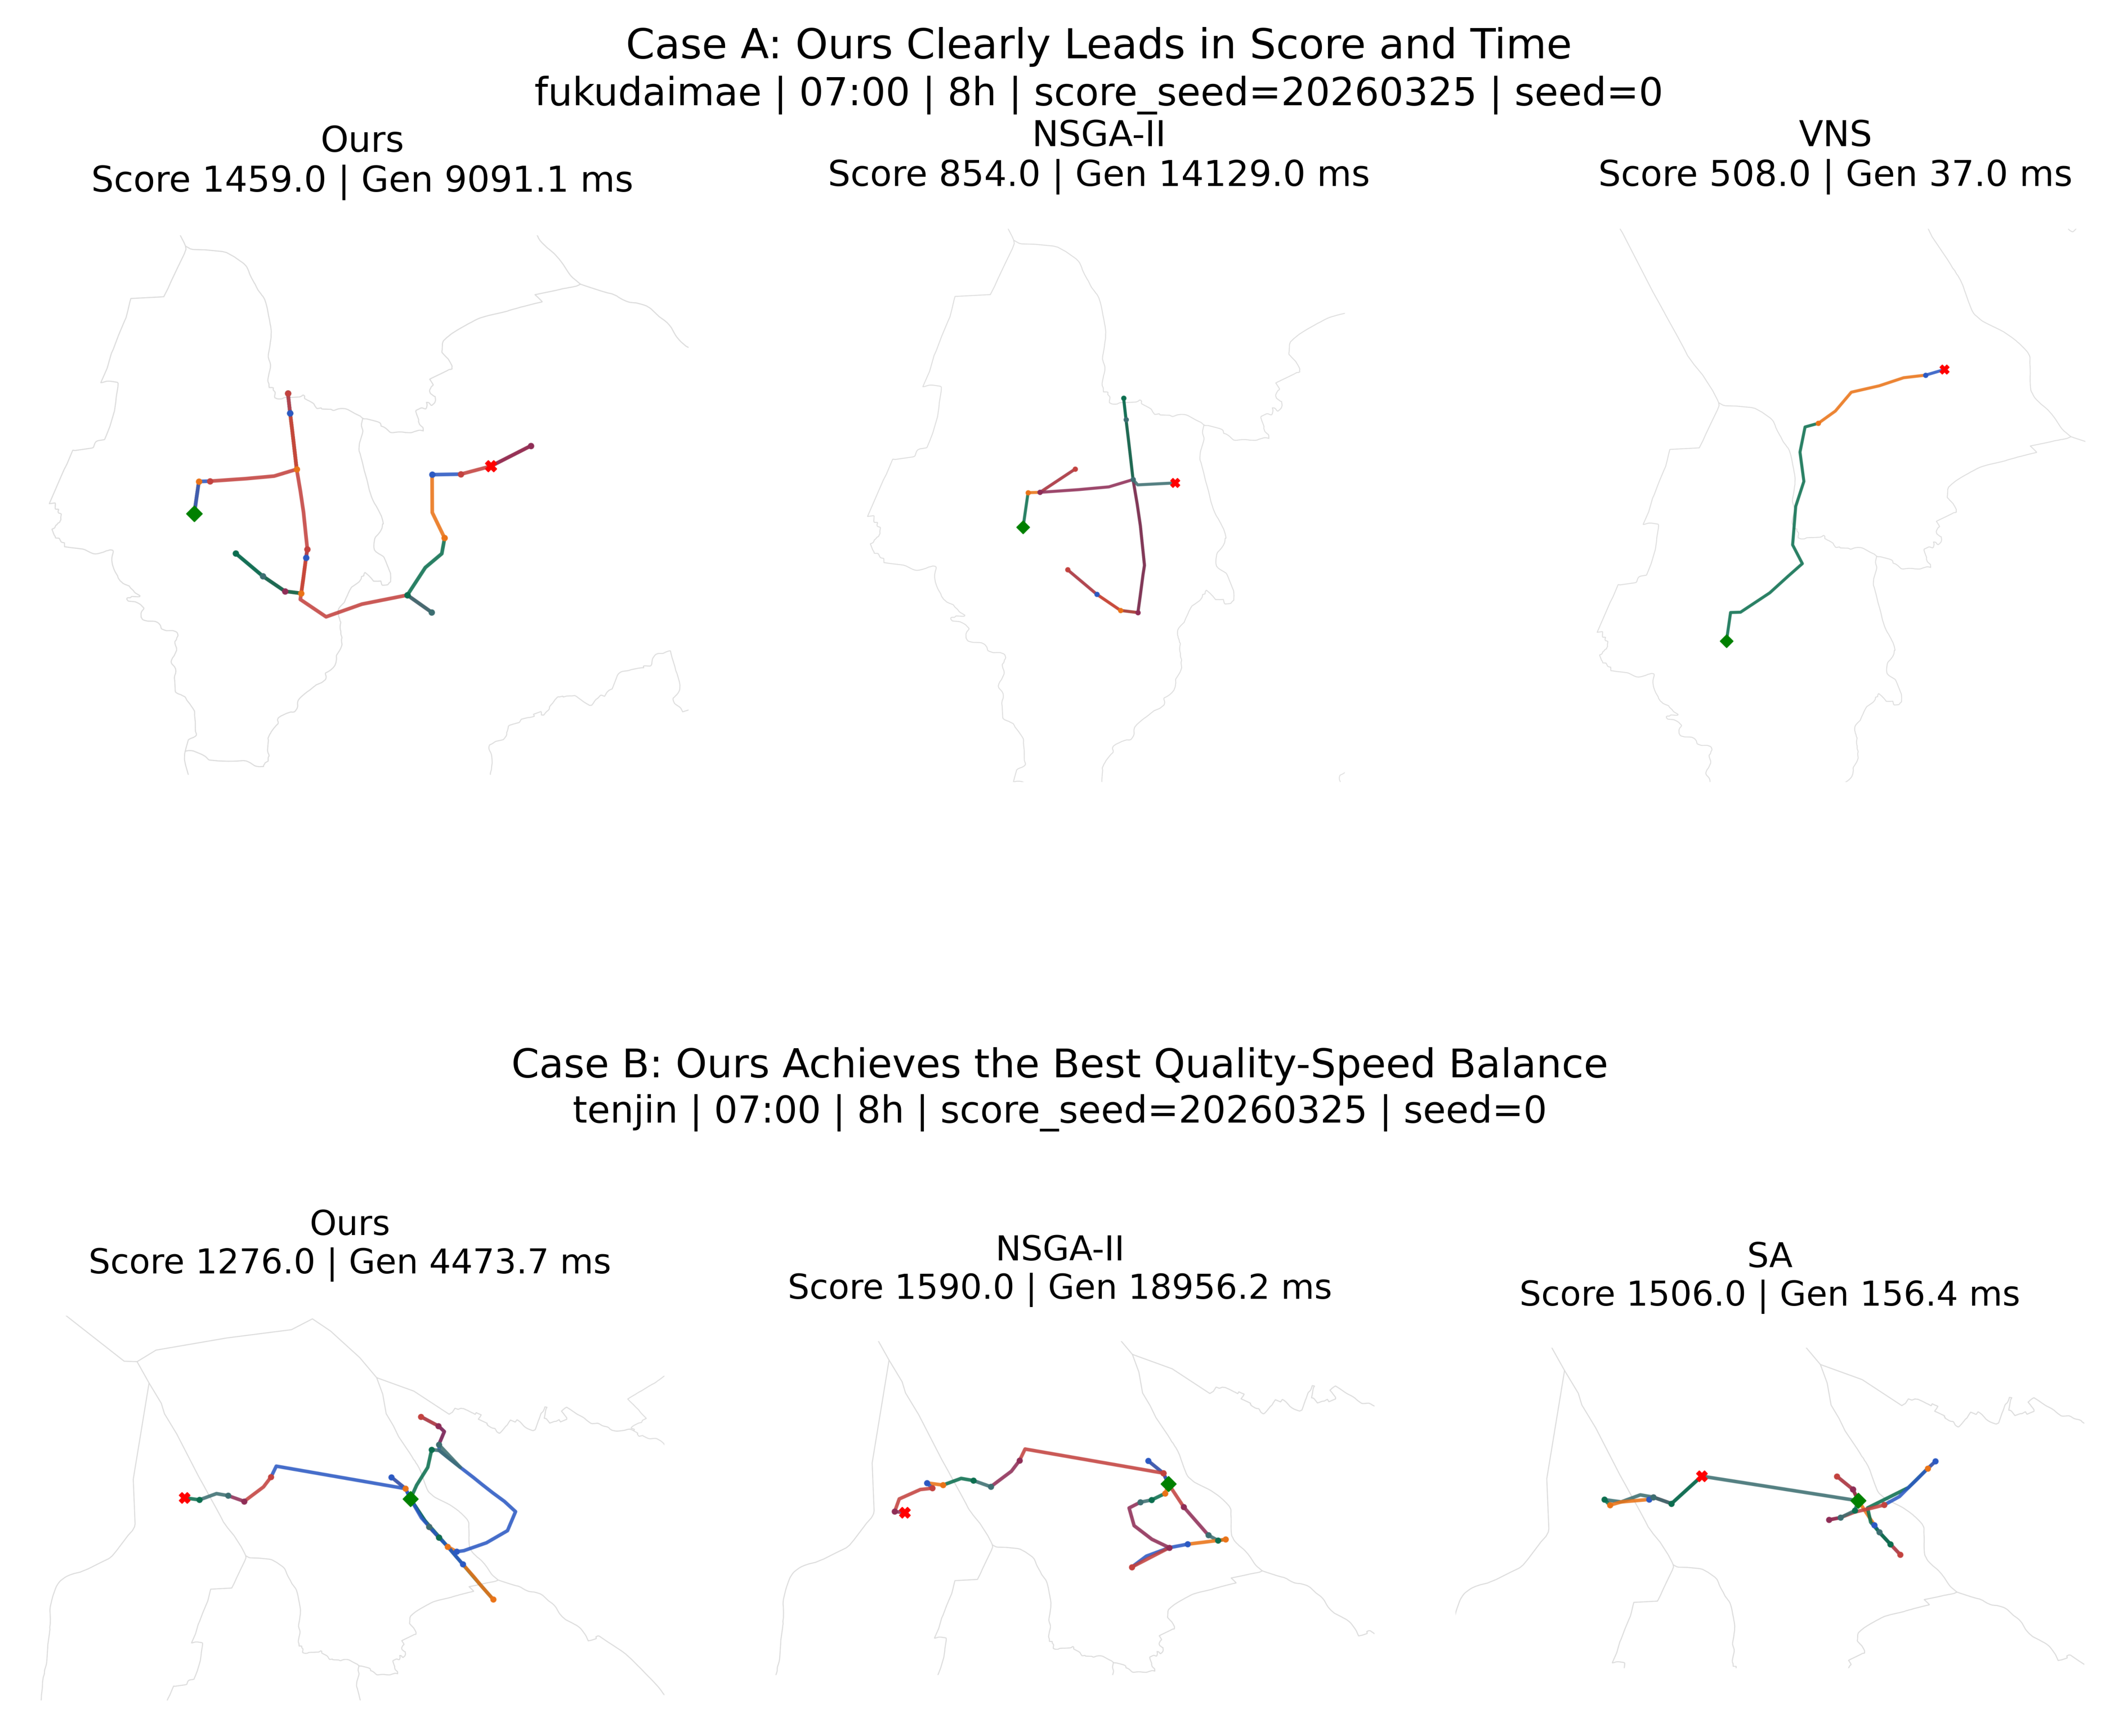
\includegraphics[width=\linewidth]{figures/exp4/exp4_main_cases.png}
    \caption{実験4の main cases．上段が Case A，下段が Case B である}
\end{figure}

\begin{figure}[H]
    \centering
    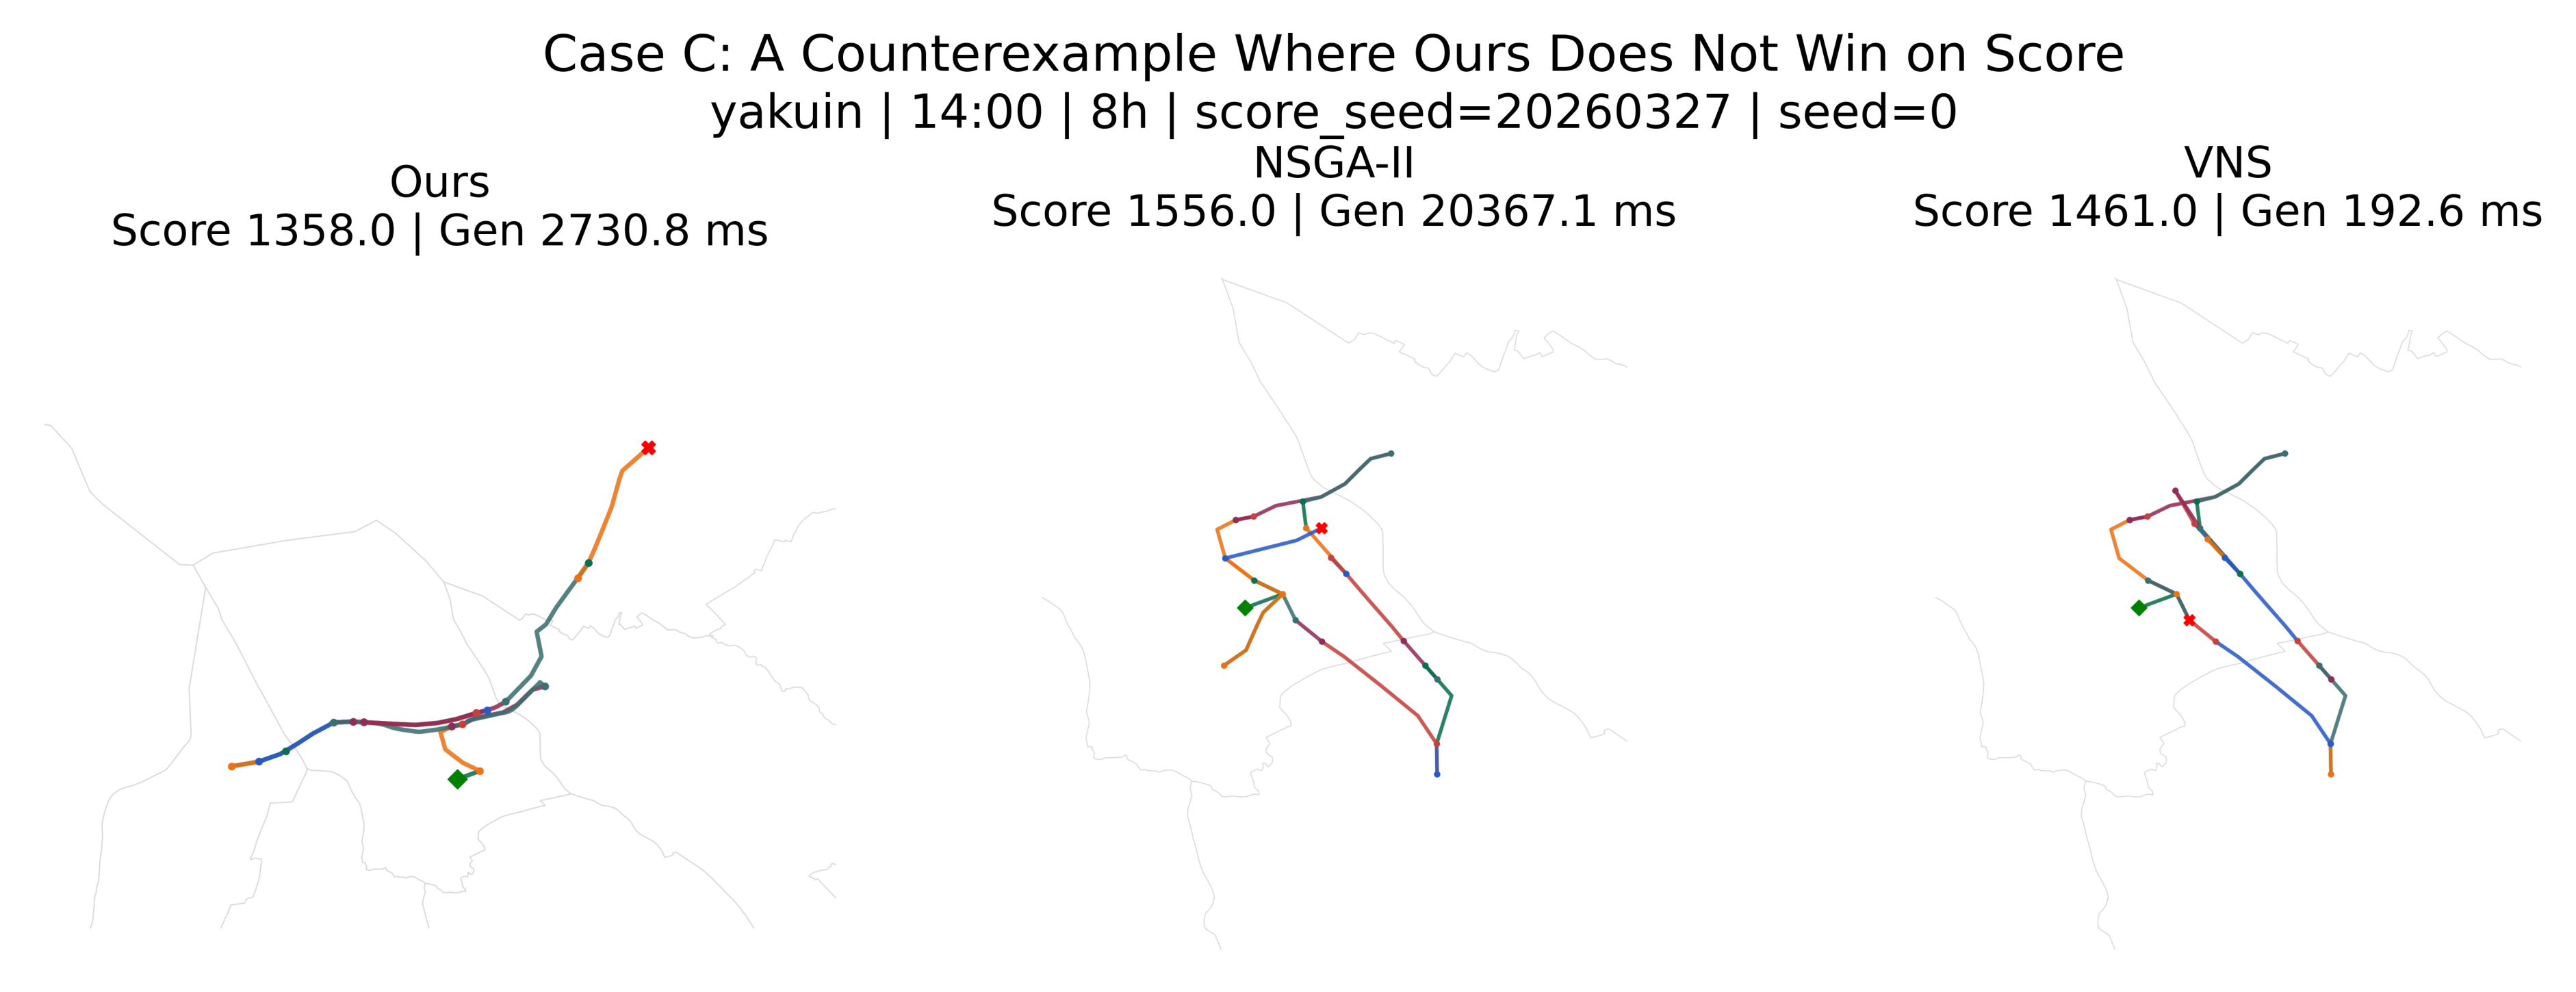
\includegraphics[width=\linewidth]{figures/exp4/exp4_appendix_cases.png}
    \caption{実験4の appendix case．Case C を反例として残し，Ours が every query で最高 score とは限らないことを明示する}
\end{figure}

\subsection*{結果の解釈}
Case A は最もわかりやすい success case です．
Ours は NSGA-II より stop score で大きく勝ち，
runtime でも短いので，
「Ours が本当に両軸で勝てる query がある」ことを視覚的に見せられます．

Case B は，今回の論文でむしろ重要な例だと思っています．
ここでは Ours が最高 score ではありませんが，
NSGA-II ほど遅くなく，
SA ほど極端に score を犠牲にもしていません．
つまり，
実験3で言っている quality-speed balance の主張を，
route の形と数値を並べて説明できる case です．

Case C は，あえて残した方がよい limitation だと思っています．
Ours は速いですが最高 score は逃しているので，
ここを appendix 側に置くことで，
「Ours は全 query で universal best」とは言っていないことを明確にできます．

\end{document}
